\documentclass[../main.tex]{subfiles}

\begin{document}


\practica{Conexión con periféricos externos - Display y drivers}

    \subsection{Objetivos}
        \begin{itemize}
            \item Realizar conexión con periféricos externos, en concreto el display.
            \item Programar un driver sencillo para controlar el pintado.
        \end{itemize}

    \subsection{Fundamentos teóricos}
        
        Cualquier procesador, sea del tipo que sea, se acompaña siempre, además de los periféricos internos, de periféricos externos. De lo contrario, la interfaz de comunicación con el usuario resultaría imposible. Desde simples pines con los que comunicar vía \PER{UART}, como ya hemos visto, hasta sistemas complejos como los que veremos en esta práctica. Las conexiones de las que dispone nuestra placa \BOARD se pueden observar en \BRDMAN[5], aunque las reproducimos en la \Cref{fig:board_connections} para facilitar la consulta.

        \begin{figure}
            \centering
            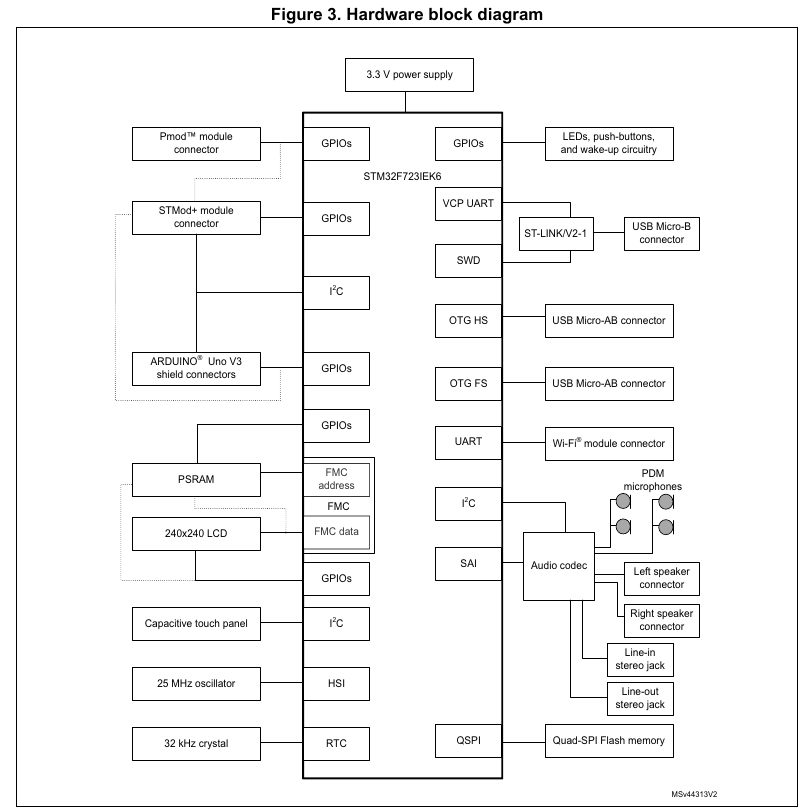
\includegraphics[width=\textwidth]{res/board_block_diagram.png}
            \caption{Diagrama de bloques de la placa \BOARD}
            \label{fig:board_connections}
        \end{figure}

        En concreto, observando dicha imagen, vemos que el display (a la izquierda) se conecta con la placa a través de GPIOs, y un periférico interno conocido como \PER{FMC}. El \PER{FMC} o \emph{Flexible Memory Controller} (\REFMAN[12]) es un periférico que permite gestionar la conexión con memorias externas de diferentes tipos (SDRAM, NAND flash, PSRAM, NOR flash...) además de dispositivos basados en memorias, como los displays (que guardan la imagen de manera similar a como una memoria guarda datos). Esto libera la memoria interna del \MCU para poder guardar programas, en lugar de pesadas imágenes.
        
        Dichas conexiones requieren el manejo simultáneo de múltiples pines de entrada y salida, lo cual sería imposible de realizar directamente con el procesador. Por tanto, este periférico \PER{FMC} permite, con una configuración apropiada, gestionar las transferencias de datos de manera autónoma. Podemos efectivamente comprobar que efectivamente el display está conectado al \PER{FMC} observando \BRDMAN[5.14]. Adicionalmente, en \BRDMAN[6.7], nos dice qué pines se utilizan para las conexiones. (Estos nombres no son directamente los puertos GPIO de la placa, que se pueden consultar en \BRDMAN[Table 19].) Cruzando estos datos con \REFMAN[12.3], podemos ver qué señales concretas se utilizan para esta placa concreta.

        Pero hay una peculiaridad, y es que el \PER{FMC} en este caso no se comunica directamente con el display, sino que, de por medio, hay un chip controlador \LCDMAN. Este chip está encargado de recibir comandos a través del \PER{FMC}, configurando la memoria del display, así como sus características. Así pues, toda la información o comandos que queramos pasar al display deberán pasar por el \PER{FMC}.

        Adicionalmente, el propio panel LCD (modelo \texttt{\textbf{FRD154BP2901}} de \emph{Frida}) cuenta con unas conexiones especiales que no controla el \LCDMAN. Estas conexiones, concretamente, son tres pines (\BRDMAN[Table 14]): PH7 (resetea el panel), PH11 (se encarga de encender la luz trasera) y PC8 (Interrupción de Tear Effect, no hace falta utilizar este último). 

        Es decir, que parte del control lo haremos directamente, y parte a través del periférico \PER{FMC}. Podemos ver todas estas conexiones de manera simplificada en \Cref{fig:hardware_connections}.

        \begin{figure}[htbp]
        \centering
        \begin{tikzpicture}[
            node distance=1.5cm and 2cm,
            block/.style={rectangle, draw=blue!70, fill=blue!10, thick, minimum width=2.5cm, minimum height=1.2cm, align=center, rounded corners=2pt},
            subblock/.style={rectangle, draw=gray!80, fill=white, thick, minimum width=2cm, minimum height=0.8cm, align=center, font=\small},
            group/.style={draw=black!60, dashed, thick, inner sep=0.3cm, rounded corners=5pt},
            line/.style={draw, -Stealth, thick},
            bus/.style={draw, -Stealth, ultra thick, double}
        ]

            % MCU y periféricos
            \node[block] (mcu) {\textbf{STM32F723e}\\\small(MCU)};
            \node[subblock, below=0.5cm of mcu] (fmc) {\PER{FMC}};
            \node[subblock, below=0.5cm of fmc] (gpio) {GPIOs\\\small(PH11, PH7)};

            % Contenedor MCU
            \node[group, fit=(mcu) (fmc) (gpio), label=above:\textbf{Procesador}] (board) {};

            % Controlador Display
            \node[block, right=3.5cm of mcu] (ctrl) {\textbf{ST7789H2}\\\small(Controlador LCD)};

            % Panel LCD Físico
            \node[block, right=2.5cm of ctrl] (panel) {\textbf{FRD154BP2901}\\\small(Panel LCD Frida)};

            % Contenedor Módulo Display
            \node[group, fit=(ctrl) (panel), label=above:\textbf{Módulo Display LCD}] (display) {};

            % Conexiones Bus FMC
            \draw[bus] (fmc.east) -| node[below, font=\scriptsize] {Bus de Datos/Control} (ctrl.south);

            % Conexiones Directas GPIO
            \draw[line] ($(gpio.east)-(0,0.3)$) -| node[near start, below, font=\scriptsize] {PH11 (Backlight)} ($(panel.south)+(0.3,0)$);
            \draw[line] ($(gpio.east)+(0,0.3)$) -| node[near start, below, font=\scriptsize] {PH7 (Reset HW)} ($(panel.south)-(0.3,0)$);

            % Conexión Interna Controlador -> Panel
            \draw[bus] (ctrl) -- node[above, font=\scriptsize] {Driver Lines} node[below, font=\scriptsize] {(RGB/Gate/Source)} (panel);

        \end{tikzpicture}
        \caption{Diagrama de conexiones entre la MCU STM32F723, el controlador ST7789H2 y el panel LCD.}
        \label{fig:hardware_connections}
        \end{figure}

        Ahora, con todas las conexiones hechas, hay que activar el panel. Para activar periféricos, se siguen ciertas secuencias de inicialización que ponen el hardware en un estado inicial. Aunque la documentación no es muy clara, si os fiáis de vuestro profesor, y no habéis abandonado la asignatura por dificultad (espero que no, si es así contactadme), el proceso no es excesivamente complicado. Habrá primero que activar el panel a través de los pines de conexión directa (básicamente, resetearlo), y luego activar el controlador \LCDMAN utilizando comandos enviados por el \PER{FMC}. En concreto, la secuencia necesaria de encendido es:

        \begin{enumerate}
            \item Encender la luz trasera del display desde el pin PH11 (esto es opcional, pero querremos ver la pantalla, no?).
            \item Aplicar la secuencia de reset en \texttt{PH7}: \texttt{0} (esperar 5\,ms) $\to$ \texttt{1} (esperar 10\,ms) $\to$ \texttt{0} (esperar 20\,ms) $\to$ \texttt{1} (esperar 10\,ms).
            \item Con el panel encendido, toca el turno al controlador, al que tenemos que mandar un comando de \texttt{SWRESET}. 
                \begin{enumerate}
                    \item Mandar un comando de \texttt{SLEEP\_IN} \LCDMAN[9.1.11] para asegurar que el panel está desactivado. La documentación obliga a esperar 5ms, esperamos 10ms para asegurar.
                    \item Mandar un comando de \texttt{SWRESET} \LCDMAN[9.1.2] para resetear el panel. La documentación obliga a esperar 120ms, esperamos 200ms para asegurar.
                    \item Mandar un comando de \texttt{SLEEP\_OUT} \LCDMAN[9.1.12] para activar el panel. La documentación obliga a esperar 5ms, pero como menciona 120ms también, esperamos ese tiempo para asegurar. 
                \end{enumerate}
        \end{enumerate}

        Lo más interesante aquí es que estos comandos que debe recibir el panel LCD, se van a enviar a través del \PER{FMC}. Es decir, que estamos delegando la configuración en este periférico versátil, en lugar de tener que hacerlo nosotros a través de los aproximadamente 30 pines que lo controlan. Y ahora, cómo funciona todo esto?

        \subsubsection{Funcionamiento del periférico FMC}

            El periférico \PER{FMC} funciona, a ojos del programador, como una extensión de la memoria RAM del sistema. En lugar de requerir un protocolo de comunicación complejo con llamadas a funciones de transmisión bit a bit, el \PER{FMC} mapea el controlador externo directamente en el mapa de memoria del microcontrolador (\REFMAN[12.4]).

            Esto significa que escribir o leer en el controlador de pantalla es tan sencillo como hacer una operación de escritura en una dirección de memoria (\emph{pointer dereferencing}) en C. El propio hardware del \PER{FMC} se encarga de traducir esa escritura en las señales eléctricas apropiadas (bus de datos, activación de \texttt{CS}, pulsos de \texttt{WR/RD}, etc.) a través de los pines GPIO asignados. En este caso, únicamente se mapean dos direcciones: \texttt{REG} (para indicar el registro o comando del periférico) y \texttt{RAM} (para indicar el valor que se escribe):

            \begin{lstlisting}
                typedef struct
                {
                    volatile uint16_t REG;
                    volatile uint16_t RAM;
                } FMC_CONTROLLER_TypeDef;

                #define FMC_BANK2       	((FMC_CONTROLLER_TypeDef *) FMC_BANK2_BASE_ADDR)

                static inline void FMC_BANK2_WriteReg(uint8_t Reg)
                {
                    /* Write 16-bit Index, then write register */
                    FMC_BANK2->REG = Reg;
                    __DSB();
                }

                static inline void FMC_BANK2_WriteData(uint16_t Data)
                {
                    /* Write 16-bit Reg */
                    FMC_BANK2->RAM = Data;
                    __DSB();
                }
            \end{lstlisting}

            Para comunicarse con el \LCDMAN, el \PER{FMC} utiliza una interfaz de tipo 8080/6800 paralela de tipo SRAM. En esta interfaz, hay una línea de control crítica conocida como A0 (o Data/Command) (\BRDMAN[Table 14]):
            \begin{itemize}
                \item Cuando la línea A0 está a nivel bajo (\texttt{0}), la transferencia se interpreta como un comando o instrucción para el controlador.
                \item Cuando la línea A0 está a nivel alto (\texttt{1}), la transferencia se interpreta como datos (parámetros del comando o colores de los píxeles).
            \end{itemize}

            Gracias al mapeo en memoria, en este caso en el banco 2 (\texttt{BANK2}) del \PER{FMC}, diferenciar entre enviar un comando o un dato es tan simple como escribir en dos direcciones de memoria consecutivas dentro del rango asignado al \PER{FMC}. La dirección base (\texttt{REG}) enviará la línea A0 a \texttt{0} (Comandos), mientras que la siguiente (\texttt{RAM}) enviará A0 a \texttt{1} (Datos).

        \subsubsection{Funcionamiento del controlador ST7789H2}

            El chip \LCDMAN es el ``cerebro'' interno del panel LCD. Su función principal es mantener la imagen visible en la pantalla refrescando continuamente los píxeles físicos, liberando por completo al \MCU.

            Para lograr esto, el \LCDMAN contiene una memoria RAM interna de $240 \times 320$ localizaciones de memoria, que se configura mediante secuencias de comandos y datos concretas a través del \PER{FMC}. El flujo general de trabajo con este chip consta de tres etapas:

            \begin{enumerate}
                \item \textbf{Configuración e Inicialización:} Tras la secuencia de reset, se le envían comandos mediante el \PER{FMC} para definir el formato de color (por ejemplo, RGB565 de 16 bits por píxel), orientación de la pantalla (lectura vertical u horizontal), etc.
                \item \textbf{Definición de Ventana de Trabajo:} Antes de pintar, se envía un comando de dirección de columnas (\texttt{CASET}, \LCDMAN[9.1.20]) y de filas (\texttt{RASET}, \LCDMAN[9.1.21]). Esto le dice al \LCDMAN en qué sub-región o rectángulo de la pantalla vamos a escribir.
                \item \textbf{Escritura de Píxeles:} Una vez delimitada la zona, se envía el comando de escritura en memoria (\texttt{RAMWR}, \LCDMAN[9.1.22]). A partir de ese momento, cada dato enviado por el \PER{FMC} corresponderá al color de un píxel (se pueden enviar varios en ráfaga). El propio controlador incrementa automáticamente la dirección de memoria interna píxel a píxel, llenando la ventana definida de izquierda a derecha y de arriba a abajo.
            \end{enumerate}

            Es decir, el procesador escribe los colores a cada píxel en la memoria mediante el \PER{FMC}, el \LCDMAN los almacena en su RAM interna y sus circuitos de control (drivers (no confundir con driver software)) convierten esos valores digitales en las tensiones físicas que configuran el display \texttt{\textbf{FRD154BP2901}}. Un diagrama mostrando este funcionamiento se observa en la \Cref{fig:memory_mapping}.

        \begin{figure}[htbp]
        \centering
        \begin{tikzpicture}[
            node distance=0.5cm and 1.5cm,
            font=\sffamily\small,
            box/.style={draw=black!70, thick, rounded corners=3pt, align=center, fill=white},
            membox/.style={draw=blue!80, thick, fill=blue!5, minimum width=3.2cm, align=center},
            fmcbox/.style={draw=orange!80, thick, fill=orange!5, minimum width=2.8cm, minimum height=3.5cm, align=center},
            lcdbox/.style={draw=green!60!black, thick, fill=green!5, minimum width=3.5cm, minimum height=3.5cm, align=center},
            arrow/.style={-Stealth, thick},
            bus/.style={double, -Stealth, thick}
        ]

            % 1. MAPA DE MEMORIA DEL MCU
            \node[font=\bfseries] (mcu_title) {1. Mapa Memoria MCU};
            
            \node[membox, below=1.025cm of mcu_title] (ram) {\texttt{FMC\_BANK2->RAM}\\ \scriptsize (Base + 0x02)};
            \node[membox, below=0.0cm of ram] (reg) {\texttt{FMC\_BANK2->REG}\\ \scriptsize (Base + 0x00)};
            \node[draw=gray, dashed, fit={(ram) (reg)}, label=below:\scriptsize Espacio Memoria FMC] (mcu_group) {};

            % 2. HARDWARE FMC
            \node[font=\bfseries, right=1cm of mcu_title] (fmc_title) {2. Periférico FMC};
            \node[fmcbox, below=0.3cm of fmc_title] (fmc_hw) {
                \textbf{Traductor HW}\\[0.3em]
                Genera bus paralelo:\\
                $\bullet$ Bus Datos (D0-D15)\\
                $\bullet$ Lógica Write/Read\\
                $\bullet$ Lógica Chip Select
            };

            % 3. CONTROLADOR DISPLAY (ST7789H2)
            \node[font=\bfseries, right=1cm of fmc_title] (lcd_title) {3. Controlador ST7789H2};
            
            \node[lcdbox, below=0.3cm of lcd_title] (lcd_hw) {};
            \node[box, fill=green!20, draw=green!50!black, minimum width=2.4cm] at (lcd_hw.north) [yshift=-0.8cm] (cmd_dec) {\textbf{Comando/Registro}\\\scriptsize Control de pantalla};
            \node[box, fill=purple!10, draw=purple!50!black, minimum width=2.4cm, minimum height=1.2cm] at (lcd_hw.south) [yshift=0.9cm] (gram) {\textbf{RAM Interna}\\\scriptsize $240 \times 320$ píxeles\\\scriptsize (Matriz de color)};

            % FLECHAS Y CONEXIONES (MCU -> FMC)
            \draw[arrow] (reg.east) -- node[above, font=\tiny] {Escritura} node[below, font=\tiny] {\texttt{REG}} ($(fmc_hw.west)+(0,-0.5)$);
            \draw[arrow] (ram.east) -- node[above, font=\tiny] {Escritura} node[below, font=\tiny] {\texttt{RAM}} ($(fmc_hw.west)+(0,0.5)$);

            % FLECHAS Y CONEXIONES (FMC -> DISPLAY)
            % Linea A0 = 0 (Comando)
            \draw[arrow, color=red!80!black] ($(fmc_hw.east)+(0,0.8)$) -- 
                node[above, font=\scriptsize\bfseries] {A0 = 0} 
                node[below, font=\tiny] {(Línea D/C baja)} (cmd_dec.west);

            % Linea A0 = 1 (Datos/GRAM)
            \draw[arrow, color=blue!80!black] ($(fmc_hw.east)+(0,-0.8)$) -- 
                node[above, font=\scriptsize\bfseries] {A0 = 1} 
                node[below, font=\tiny] {(Línea D/C alta)} (gram.west);

            \draw[arrow] (cmd_dec.south) -- node[right, font=\tiny] {Posición} (gram.north);

            % ANOTACIÓN EXPLICATIVA INFERIOR
            \node[draw=orange!50, fill=orange!10, rounded corners, inner sep=5pt, below=0.6cm of fmc_hw, font=\scriptsize, align=center] {
                La dirección elegida en C conmuta el pin \textbf{A0} automáticamente.\\
                \textbf{\texttt{REG}} $\rightarrow$ Pin A0 a \texttt{0} $\rightarrow$ Apunta a Comandos.\\
                \textbf{\texttt{RAM}} $\rightarrow$ Pin A0 a \texttt{1} $\rightarrow$ Apunta a Datos / RAM.
            };

        \end{tikzpicture}
        \caption{Mapeo de memoria a través del FMC hacia la lógica y RAM interna del ST7789H2}
        \label{fig:memory_mapping}
        \end{figure}


    \subsection{Desarrollo de la práctica}

        Para esta práctica, vamos a partir del código final de \texttt{main.c} al que queremos llegar. Básicamente, inicializaremos todos los elementos necesarios (el panel LCD, el periférico \PER{FMC}, y el controlador \LCDMAN[]), antes de dibujar algo sencillo en la pantalla. Se incluye además un pequeño código para poner píxeles aleatorios y ver que de verdad está funcionando:

        \begin{lstlisting}
            // Definimos una variable global para la semilla (debe ser distinta de 0)
            static uint32_t estado_rng = 123456789;

            // Genera un entero sin signo de 32 bits (0 a 4,294,967,295)
            uint32_t rand32(void) {
                uint32_t x = estado_rng;
                x ^= x << 13;
                x ^= x >> 17;
                x ^= x << 5;
                return estado_rng = x;
            }

            int main(void)
            {
                LCD_Init();
                FSMC_Init();
                ST7789H2_INIT();

                /* Clear the LCD */
                for (int i = 0; i < 240; i++)
                    for (int j = 0; j < 240; j++)
                        ST7789H2_WritePixel(i, j, LCD_COLOR_WHITE);


                for (int i = 50; i < 60; i++)
                    for (int j = 50; j < 60; j++)
                        ST7789H2_WritePixel(i, j, LCD_COLOR_RED);


                while(1)
                {
                    uint32_t rnd = rand32();
                    ST7789H2_WritePixel((rnd >> 24) & 0xff, (rnd >> 16) & 0xff, rnd & 0xffff);
                }
            }
        \end{lstlisting}

        Yendo por orden, lo primero es inicializar el panel LCD. Lo primero es configurar los pines de conexión directa (de reset, interrupción (que no utilizaremos) y luz trasera). Posteriormente, aplicaremos la secuencia de inicialización del panel.

        \begin{lstlisting}
            void LCD_Pins_Init() {
                /* Initialize LCD special pins GPIOs */
                /* LCD_RESET GPIO configuration */
                RCC_AHB1ENR->bits.GPIOHEN = 1;
                GPIO_CONFIG(GPIOH, 7, GPIO_MODE_OUTPUT, GPIO_OTYPE_PP, GPIO_OSPEED_HIGH, GPIO_PUPD_NONE, 0);
                /* LCD_TE GPIO configuration */
                RCC_AHB1ENR->bits.GPIOCEN = 1;
                GPIO_CONFIG(GPIOC, 8, GPIO_MODE_INPUT, GPIO_OTYPE_PP, GPIO_OSPEED_HIGH, GPIO_PUPD_NONE, 0);
                /* LCD_BL_CTRL GPIO configuration */
                RCC_AHB1ENR->bits.GPIOHEN = 1;
                GPIO_CONFIG(GPIOH, 11, GPIO_MODE_OUTPUT, GPIO_OTYPE_PP, GPIO_OSPEED_LOW, GPIO_PUPD_NONE, 0);
            }

            void LCD_Startup_Seq() {
                /* Backlight enable */
                GPIO_PIN_WRITE(GPIOH, 11, GPIO_STATE_ONE);

                /* Apply hardware  */
                //... completar escribir en el pin de reset la secuencia de activación
                //... utiliza la función DELAY para las esperas
            }

            void LCD_Init() {
                LCD_Pins_Init();
                LCD_Startup_Seq();
            }
        \end{lstlisting}

        Una vez iniciado el panel, lo siguiente es activar el \PER{FMC}. La configuración es bastante complicada y ya está hecha en el código proporcionado de base. Se recomienda echar un vistazo. En resumen, lo que hacemos es activar primero todos los pines requeridos por el controlador, y luego configurar el modo de conexión con la memoria, así como las características de temporización del bus.

        Finalmente, se configura el controlador del display, enviando comandos directamente desde el \PER{FMC}. El código se encuentra en \texttt{ST7789h2.h}, y hay que completar algunas partes para hacerlo funcionar completamente. En concreto:

        En la función \texttt{ST7789H2\_INIT}, al principio, debemos inicializar el controlador, mandando los comandos adecuados:

        \begin{lstlisting}
            /* Sleep In Command */
            ST7789H2_WriteReg(ST7789H2_SLEEP_IN, (uint8_t*)NULL, 0);
            /* Wait for 10ms */
            DELAY(10);

            //... completar mandar el comando de RESET, seguido de una pausa de 200ms
            //... completar mandar el comando de SLEEP_OUT, seguido de una pausa de 120ms
        \end{lstlisting}

        También deberemos crear la función \texttt{DISPLAY\_ON} para encender el display:

        \begin{lstlisting}
            void ST7789H2_DisplayOn(void)
            {
                //... completar mandar el comando DISPLAY_ON
                //... completar mandar el comando SLEEP_OUT
            }
        \end{lstlisting}

        Con esto ya deberíamos tener el display funcionando! El código debería borrar el display a blanco (tardará un poco), pintar un cuadrado rojo, y luego empezar a dibujar cuadrados de colores aleatoriamente.

        Amplía ahora la librería con funciones de dibujado de líneas, rectángulos, círculos... Así podrás tener mucho más control (y hacer de manera más fácil) el dibujado en pantalla. También te puede servir para más tarde desarrollar aplicaciones con interfaces bien chulas.
    
    \subsection{Para hacer más} 
        
        Explora la documentación del display para estudiar las maneras más rápidas de pintar la pantalla (por líneas en lugar de píxeles, por ejemplo). También puedes aumentar la velocidad del procesador cambiando su frecuencia de reloj de los 16MHz por defecto a más de 200MHz para conseguir mayor velocidad.

\end{document}



%    1) Initialize special LCD pins (RST on PH7, TE on PC8, BL PH11)
%2) Todo lo del FMC

%FMC pins
%PD10, PD9, PD8, PE15, PE14, PE13, PE12, PE11, PE10, PE9, PE8, PE7, PD1, PD0, PD15, PD14

%FMC NOE, NWE
%PD4, PD5

%FMC RS FMC_A0
%PF0

%FMC NCS
%PG9

%LCD RESET 
%PH7